\newcommand{\IncludePerfProfSubFigures}[1]{
	\begin{subfigure}{0.45\textwidth}
		\centering
		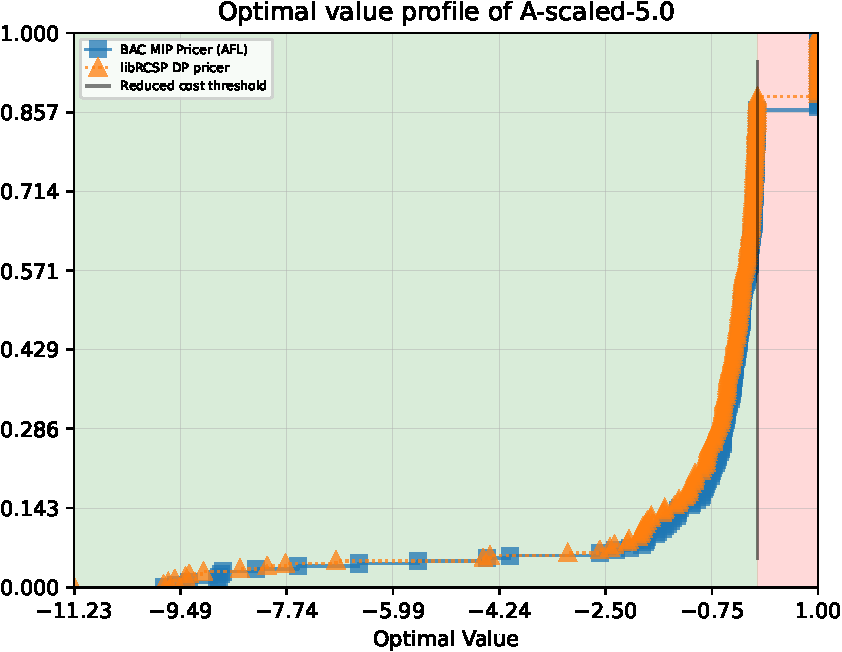
\includegraphics[width=1.0\linewidth]{./Imgs/perfprofs/#1/OptimalValue_plot.cropped.pdf}
	\end{subfigure}
	\hfill
	\begin{subfigure}{0.45\textwidth}
		\centering
		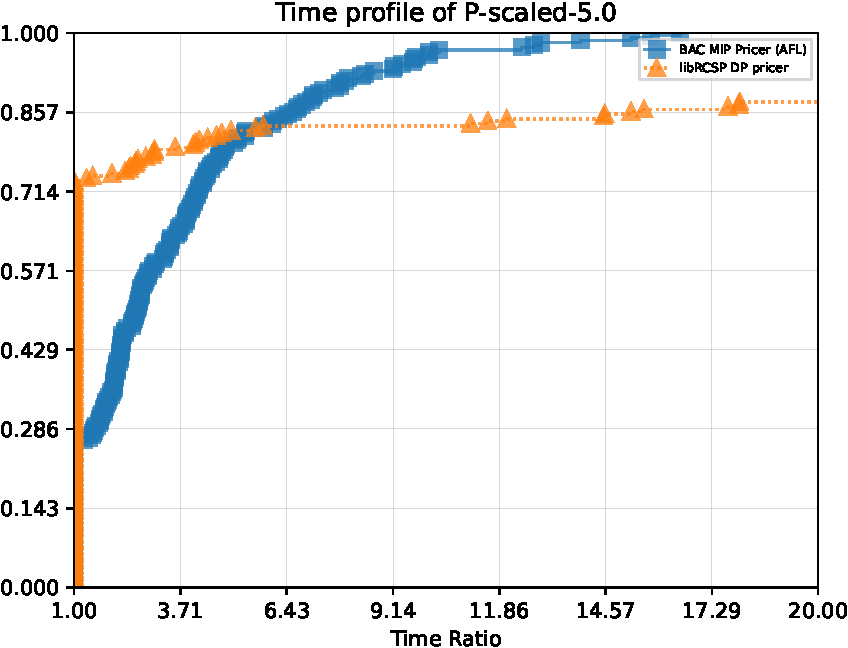
\includegraphics[width=1.0\linewidth]{./Imgs/perfprofs/#1/Time_plot.cropped.pdf}
	\end{subfigure}%
}

\newcommand{\PerfprofFigureCaptionOne}[1]{
	Empirical study comparing the pricing performance of the proposed BAC-pricer to the labeling algorithm
	of \textcite{pessoa2020generic} on the \texttt{#1} test set.
	On the left, the cost profile representing the optimal value found by each method.
	On the right, the time profile measuring the time ratio of the two approaches.
	Each row represents a different inflation scale factor $s$.
	From top to bottom: $s = 1, 2 \text{ and } 4$.
}

\newcommand{\PerfprofFigureCaptionTwo}[1]{
	Continuation of \cref{fig:perpfrofs-batch2-#1-part1} testing even further
	inflation scale factors: $s = 5, 8, 10 \text{ and } 20$.
}

\newcommand{\PerfprofFiguresPartOne}[1]{
	\begin{figure}[t]
		\IncludePerfProfSubFigures{#1-scaled-1.0}
		\vspace{2.5mm}

		\IncludePerfProfSubFigures{#1-scaled-2.0}
		\vspace{2.5mm}

		\IncludePerfProfSubFigures{#1-scaled-4.0}

		\caption{\PerfprofFigureCaptionOne{#1}}
		\label{fig:perpfrofs-batch2-#1-part1}
	\end{figure}
}

\newcommand{\PerfprofFiguresPartTwo}[1]{
	\begin{figure}[t]
		\IncludePerfProfSubFigures{#1-scaled-5.0}
		\vspace{2.5mm}

		\IncludePerfProfSubFigures{#1-scaled-8.0}
		\vspace{2.5mm}

		\IncludePerfProfSubFigures{#1-scaled-10.0}
		\vspace{2.5mm}

		\IncludePerfProfSubFigures{#1-scaled-20.0}

		\caption{\PerfprofFigureCaptionTwo{#1}}
		\label{fig:perpfrofs-batch2-#1-part2}
	\end{figure}
}

\newcommand{\PerfprofFigures}[1]{
	\PerfprofFiguresPartOne{#1}

	\PerfprofFiguresPartTwo{#1}

}

\forcsvlist{\PerfprofFigures}{E,F,A,B,P}
